%% This is an example first chapter.  You should put chapter/appendix that you
%% write into a separate file, and add a line \include{yourfilename} to
%% main.tex, where `yourfilename.tex' is the name of the chapter/appendix file.
%% You can process specific files by typing their names in at the 
%% \files=
%% prompt when you run the file main.tex through LaTeX.

\chapter{Methodology}
This chapter describes the approaches that are planned and outlined before starting the actual implementation. The primary goal of the thesis is to identify various stages of the pipeline which can be employed for predicting pedestrian's future location. After the literature review, I was motivated by the SSD for the identification of pedestrians and locating with help of bounding box and usage of LSTM as \textit{future prediction} by considering pedestrian past move sequence as a time-series data. Also, this chapter describes some of the key concepts and terminology used in the next chapter. These are some of the key concepts in the area of machine learning with image data. Though the list of such concepts is exhaustive, the minimal terminologies and concepts are presented here.


\section{Bounding box prediction: RNN/LSTM}
Recurrent neural networks primarily are densely connected neural networks similar to a feed-forward network with a key difference; introduction of \textit{time} component in RNN. The output of a hidden layer in an RNN is \textit{fed back } into itself. With this, we can model the data which is time-dependent or sequence-dependent in nature. In programming terms, this can be represented by a fixed program taking certain inputs and some internal variables.

\begin{figure}[H]
\begin{center}
\begin{tikzpicture}[item/.style={circle,draw,thick,align=center},
itemc/.style={item,on chain,join}]
 \begin{scope}[start chain=going right,nodes=itemc,every
 join/.style={-latex,very thick},local bounding box=chain]
 \end{scope}
 \node[left=2em,item] (AL) {$A$};
 \path (AL.west) ++ (-1em,2em) coordinate (aux);
 \draw[very thick,-latex,rounded corners] (AL.east) -| ++ (1em,2em) -- (aux) 
 |- (AL.west);
 \draw[very thick,-latex] (AL.north) -- ++ (0,2em)
 node[above,item,fill=gray!10] {$h_t$};
 \draw[very thick,latex-] (AL.south) -- ++ (0,-2em)
 node[below,item,fill=gray!10] {$x_t$};
\end{tikzpicture}
\caption{Compact RNN loop}
\end{center}
\end{figure}

\newpara The above diagram depicts a compact loop form of an RNN showing a loop. An RNN can be thought of as multiple copies of the same network, each previous network passing a message to its successor. By unrolling the compact for we can visualize the RNN as below. 

\begin{figure}[H]
\begin{center}
\begin{tikzpicture}[item/.style={circle,draw,thick,align=center},
itemc/.style={item,on chain,join}]
 \begin{scope}[start chain=going right,nodes=itemc,every
 join/.style={-latex,very thick},local bounding box=chain]
 \path node (A0) {$A$} node (A1) {$A$} node (A2) {$A$} node[xshift=2em] (At)
 {$A$};
 \end{scope}
 \node[left=1em of chain,scale=2] (eq) {$=$};
 \node[left=2em of eq,item] (AL) {$A$};
 \path (AL.west) ++ (-1em,2em) coordinate (aux);
 \draw[very thick,-latex,rounded corners] (AL.east) -| ++ (1em,2em) -- (aux) 
 |- (AL.west);
 \foreach \X in {0,1,2,t} 
 {\draw[very thick,-latex] (A\X.north) -- ++ (0,2em)
 node[above,item,fill=gray!10] (h\X) {$h_\X$};
 \draw[very thick,latex-] (A\X.south) -- ++ (0,-2em)
 node[below,item,fill=gray!10] (x\X) {$x_\X$};}
 \draw[white,line width=0.8ex] (AL.north) -- ++ (0,1.9em);
 \draw[very thick,-latex] (AL.north) -- ++ (0,2em)
 node[above,item,fill=gray!10] {$h_t$};
 \draw[very thick,latex-] (AL.south) -- ++ (0,-2em)
 node[below,item,fill=gray!10] {$x_t$};
 \path (x2) -- (xt) node[midway,scale=2,font=\bfseries] {\dots};
\end{tikzpicture}
\caption{Unrolling RNN loop}
\end{center}
\end{figure}
Mathematically RNNs can be represented as below: 

\begin{equation}
	\textbf{h}_t = f_W(\textbf{h}_{t-1} + \textbf{x}_{t}) 
\end{equation}

Where \textbf{\textit{ f}} is some function with parameter \textbf{W}. \\
This same function \textbf{\textit{ f}} and same weight matrix \textbf{W} is used at every step of the computation. \\
\textit{$h_t$} is new state \\
\textit{$h_{t-1}$} is old state \\
\textit{$x_t$} input vector at time step \textit{t}\\

In a more simplified form, we can have the above function as:

\begin{equation}\label{hidden_state}
	\textbf{h}_t = \sigma (\textbf{Ux}_t + \textbf{Vh}_{t-1}) 
\end{equation}

Where \textit{U} is the input weight matrix and \textit{V} is the recurrent outputs. Timestamp denoted by \textit{t}. $\sigma$ represents an activation function e.g a \textit{tanh} or \textit{sigmoid}. If we unfold the above equation and go back three-time step we have,

\begin{equation}
	\textbf{h}_t = \sigma (\textbf{Ux}_t + \textbf{V}(\sigma(\textbf{Ux}_{t-1} + \textbf{V}(\sigma(\textbf{Ux}_{t-2})))
\end{equation}

And in general, if we unfold in n time slot back,

\begin{equation}
\textbf{h}_t = \sigma (\textbf{Ux}_t + ...( \textbf{V}(\sigma(\textbf{Ux}_{t-n+2} + \textbf{V}(\sigma(\textbf{Ux}_{t-n+1})..)))
\end{equation}

\begin{equation}
	\textbf{y}_t = (\textbf{W}_{hy}  \textbf{h}_{t}) 
\end{equation}

Where \textbf{$y_t$}  represents output at a timestamp \textit{t} \\
\textbf{$h_t$} is the hidden state, computed as in equation \ref{hidden_state}

The problem with RNN is, over a large period of time, the backpropagation gradients either explodes or vanishes. During a \textit{vanishing gradient } problem, the gradients of the network output with respect to the early layer of the network becomes extremely small, which indicates a large change in the parameters for the early layers, does not have a big effect on network output. Usually, this happens when the activation function such as \textit{sigmoid} or \textit{tanh} squash their input into a small output range non-linearly. Considering the activation function sigmoid which is defined as below,

\begin{equation}
	S(x) = \frac{1}{ 1+ e^x}
\end{equation}

Sigmoid is a special case of standard Logistic function defined as 
\begin{equation}
f(x) = \frac{L}{ 1+ e^{-k(x-x_0)}}
\end{equation}
Where \\
L: Curve's maximum value \\
k: Steepness of the curve \\
(x0 - x): value of Sigmoid's midpoint \\

A standard logistic function is called sigmoid when (k=1, x0=0, L=1) and can be viewed as below: \\
\begin{figure}[H]
	\centering
	\begin{tikzpicture}
		\begin{axis}%
			[
			grid=major,     
			xmin=-10,
			xmax=10,
			axis x line=bottom,
			ytick={0,.5,1},
			ymax=1,
			axis y line=middle,
			]
			\addplot%
			[
			blue,%
			mark=none,
			samples=200,
			domain=-6:6,
			]
			(x,{1/(1+exp(-x))});
		\end{axis}
	\end{tikzpicture}
	\caption{Sigmoid function}
	\label{fig:Sigmoid-function}
\end{figure}

Sigmoid function can be rewritten as  \\
\begin{equation}
	S(x) = (1+e^{-x})^{-1}
\end{equation}
And by taking the derivative \\
\begin{equation}
\frac{d}{dx}S(x) = \frac{d}{dx} (1+e^{-x})^{-1} \\
= \frac{e^{-x}} {(1+e^{-x})^{-2}} 
\end{equation}

Plotting the derivative of the sigmoid activation function as below, we notice that 
\begin{figure}[H]
\begin{center}
\begin{tikzpicture}
\begin{axis}%
[
grid=major,     
xmin=-10,
xmax=10,
axis x line=bottom,
ytick={0,.5,1},
ymax=1,
axis y line=middle,
]
\addplot%
[
blue,%
mark=none,
samples=100,
domain=-10:10,
]
(x,{exp(-x)/((1+exp(-x)) * (1+exp(-x)))});
\end{axis}
\end{tikzpicture}
\caption{Derivative of the sigmoid activation function}
\end{center}
\end{figure}

\comment {
\begin{figure}[H]
	\centering
	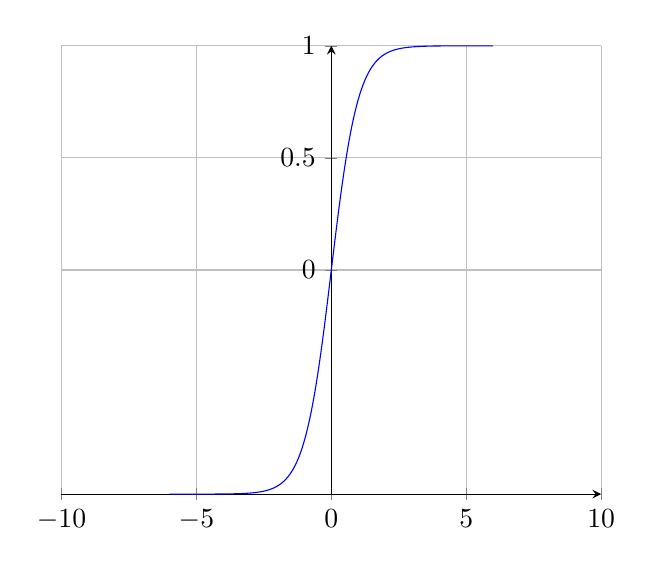
\begin{tikzpicture}
		\begin{axis}%
			[
			grid=major,     
			xmin=-10,
			xmax=10,
			axis x line=bottom,
			ytick={0,.5,1},
			ymax=1,
			axis y line=middle,
			]
			\addplot%
			[
			blue,%
			mark=none,
			samples=200,
			domain=-6:6,
			]
			(x,{(exp(2*x)-1 )/(exp(2*x)+1 )});
		\end{axis}
	\end{tikzpicture}
	\caption{Hyperbolic Tangent Function}
	\label{fig:tanh-function}
\end{figure}
}

the sigmoid derivative is well below the 1.0 in the whole range of input values. And this makes the gradients vanish quite fast as multiplying this value \footnote{value less than 1} several times for several layers, \textit{ backpropagation} brings the value close to 0.


\subsection{LSTM}
LSTM has a chain-like structure as in RNN but the repeating module has a different structure. There are four neural network layer as contrast with RNN that has a single neural network layer. The four neural network layers interact in a very special way. LSTM networks have gained acceptance for time sequence data processing, such as image captioning, action recognition, speech recognition, language translation, etc. An LSTM visually can be shown as below. 

\begin{figure}[H]
\begin{align*}
\begin{tikzpicture}[baseline=-1pt]
\node[] at (0,0) {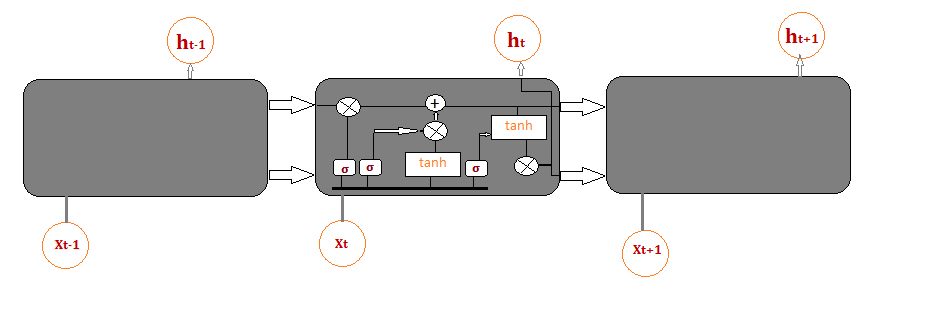
\includegraphics[scale=0.8]{LSTM3-chain1}};
\end{tikzpicture}&
\end{align*}
\begin{center}
\caption{LSTM schematic diagram}
\end{center}
\end{figure}

The core idea to LSTM is the cell state, it runs through the entire chain and performs some minor linear interaction. LSTM adds or removes information to the cell state with the help of a regulated structure called gates. Gates are represented by a neural network layer sigmoid activation and a point-wise multiplication operation.
A sigmoid generates the outputs which decides the quantity a component should be provided to the system. A value of 0 blocks the whole component and a value of 1 let the entire component through. In a basic LSTM, there are four such gates.
With the arrival of new information, the model decides the long term information which is not needed anymore and forgets it. It stores a necessary part of the new information into long-term memory. An LSTM has three such gates, that controls the cell state.
A \textbf{remember gate} is learned that takes new data and working memory as input and outputs \textit{n} bummers between 0 and 1, each determines the degree to which long-term memory element to be kept. Where 1 indicates to keep the data and 0 indicates as to forget the data entirely. A small neural network can model this \textbf{remember gate} given below. In the literature, this is also known as \textbf{forget gate}. Below mathematical expressions details various internal operation within an LSTM memory cell as discussed in the original paper of Hochreiter et.al \cite{hochreiter1997long} and simplified rewriting \cite{christopherolah}

\begin{equation}
f_t = \sigma(W_f. [h_{t-1}, x_t  ] + b_f)
\end{equation}
Where $f_t$ is the forget gate's activation vector \\
$W_f$ is the weight matrix for the forget gate \\
$h_{t-1}$ is the cell state at time (t-1) \\
$b_f$ is the bias for the forget gate

After forgetting the unnecessary information, LSTM is interested in storing the new required information in the cell state. This involves two-steps, with an \textbf{input} sigmoid layer, values that need to be updated is decided. And then a tanh layer creates a vector for new candidate values for cell state that could be added to the cell state. 

\begin{equation}
i_t = \sigma(W_i. [h_{t-1}, x_t  ] + b_i)
\end{equation}
Where $i_t$ is the input gate's activation vector 
$W_i$ is the weight matrix for the input gate \\
$h_{t-1}$ is the hidden state at time (t-1) \\
$b_i$ is the bias for the input gate

\begin{equation}
C_t\textasciitilde = tanh(W_C. [h_{t-1}, x_t ] + b_C)
\end{equation}
$C_t\textasciitilde$ represents the vector of new candidate values for the cell state
$W_C$ is the weight matrix for the tanh layer that computes the candidates\\
Both $i_t$ and $C_t\textasciitilde$ is combined to update the cell state as below.

\begin{equation}
C_t = f_t * C_{t-1} + i_t * C_t\textasciitilde
\end{equation}

Next, the output is decided based on cell state and an output gate, which decides what part of the cell state is going to output. Mathematically this can be represented as below.

\begin{equation}
o_t = \sigma(W_o. [h_{t-1}, x_t  ] + b_o)
\end{equation}
\begin{equation}
h_t = o_t  * tanh(C_t)
\end{equation}

\pagebreak

Where $o_t$ is the output gate's activation vector 
$W_o$ is the weight matrix for the output gate \\
$h_{t-1}$ is the hidden state at time (t-1) \\
$b_o$ is the bias for the output gate

There are several variants of LSTM, but the basic variant was explored and used in the scope of the thesis.

\textbf{Cell state Vs. Hidden State:}
Two entities such as \textit{cell state} and \textit{hidden state} are carried over from one-time stamp (One LSTM Cell) to another (next LSTM Cell) in an LSTM. Typically they can be represented by vectors. In an LSTM Cell, a \textit{hidden state }contains information about previous inputs. The hidden state from the previous LSTM Cell and current input are combined and processed through various gates in a particular LSTM Cell. Cell state can be regarded as the memory of the LSTM cell. There are several neural network behaves as gates and they act together to decide which information is allowed to be part of \textit{cell state}. Output-gate output and the updated cell state decide the next hidden state. \textit{Hidden states} are the output of an LSTM Cell or layer of cells and they are used for predictions.  

\subsection{LSTM Cell refinement} \label{state_refinement}

The position of the pedestrian bounding box largely depends upon the speed of the vehicle, pedestrian own speed, and the direction pedestrian makes with the camera and other social behavior such as neighboring pedestrians, stationary obstacles, etc. We propose an obvious factor that is not yet considered while predicting the future trajectory of the pedestrian by taking an important parameter into consideration; that pedestrians and vehicles always want to remain at safe distance from each other. A car lowers its speed greatly when moving at high speed to find a pedestrian near the curb waiting to cross or crossing the road. With a lesser speed and within the safe distance from pedestrian, it keeps moving slowly without halting even though pedestrians are moving in front of it.
It is also noticed that as a pedestrian moves with normal speed when a vehicle is not near and feels confident that he is in a safe zone, in contrast, he increases his speed when the vehicle approaches. So there exists a social relationship between vehicle and pedestrian and we attempted at extracting this information and make a refinement to the LSTM state. With the motivation from \cite{zhang2019sr}, we constructed a message-passing mechanism to refine the features of pedestrians by the current vehicle speed and the direction between pedestrian and vehicle (camera mounted on the vehicle). The SR module takes vehicle current speed, pedestrian movement information with respect to the vehicle, cell states and hidden states from the LSTM as input and outputs the refined cell state as shown as part of the LSTM cell below.

\begin{figure}[H]
\begin{align*}
\begin{tikzpicture}[baseline=-1pt]
\node[] at (0,0) {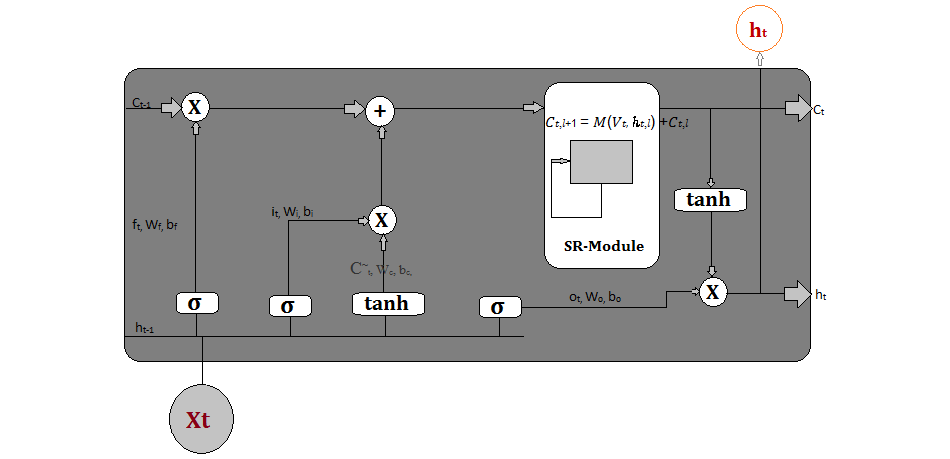
\includegraphics[scale=0.8]{LSTM3-details}};
\end{tikzpicture}&
\end{align*}
\begin{center}
\caption{LSTM-details with State Refinement module}
\end{center}
\end{figure}

%
This can be expressed mathematically as
\begin{equation}
\hat{C}^{t, l+1}= M(V^t, {h}^{t, l}) + \hat{C}^{t, l}
\end{equation}
Where $\hat{C}^{t, l+1}$ represents refined cell state at timestamp $t$ and refined iteration $l$, $V^t$ is the vehicle speed at time $t$ and rate of pedestrian location change in X-Y \\
${h}^{t, l}$ is the hidden state of the Pedestrian at timestamp $t$

After $l$ iteration of refinement in the SR module, the updated equations would be

\begin{equation}
\begin{array}{l@{}}
\hat{C}^{t}=\hat{C}^{t, l} \\
\hat{h}^{t}={g}^{o,t} \odot tanh(\hat{C}^{t}) \\
\left[ \hat{x}^{t+1}, \hat{y}^{t+1}, \hat{w}^{t+1}, \hat{h}^{t+1} \right] ^ T = W_p\hat{h}^{t}
\end{array}
\end{equation}

$\hat{w}^{t+1}$, $\hat{h}^{t+1}$ represents the bounding box width and height.
$W_p$ is the weight matrix of the output gate and \textit{p} symbolizes this is modeled for pedestrian.
%
In this case, the message passing can be formulated as below 
\begin{equation}
\hat{C}^{t, l+1}=M(P_t, V_t) +  \hat{C}^{t, l}
%{W}^{vp}\alpha_v
\end{equation}
$\hat{C}^{t, l+1}$ is the refined cell state for $(l+1)$th iteration at the $t$-timestamp \\
$M(P_t, V_t)$ is the message passing between the state of pedestrian and vehicle as described below.

We propose the message passing term $M(P_t, V_t)$ using the refinement gate as below.
\begin{equation}
M(P_t, V_t) = W^{a,p}.(g^{a,t,l} \odot {h}^{t, l} ) 
%+ \hat{C}^{t, l}
\end{equation}
Where $W^{a,p}$ is a linear transform parameter and $g^{a,t,l}$ is the refinement (includes awareness and translated bounding box position and dimension) gate vector and formulated by

\begin{equation}
g^{a,t,l} = \sigma(W^{a} [ \alpha_p, P1, {h}^{t, l} ] + b^{a} ) 
%+ \hat{C}^{t, l}
\end{equation}

Where $W^{a}$, $b^{a}$ are parameters and $\sigma$ denotes the sigmoid function, $\alpha_p$ is the awareness factor of the pedestrian and described below \ref{awareness_factor}. $P1$ is the translated position of the bounding box denoted by $(x_1, y_1, w_1, h_1)$.
$g^{a,t,l}$ selects features from ${h}^{t, l}$ by element-wise product.

So 
\begin{equation}
\hat{C}^{t, l+1}= W^{a,p}.(g^{a,t,l} \odot {h}^{t, l} )+  \hat{C}^{t, l}
%{W}^{vp}\alpha_v
\end{equation}

%Where\alpha_v is the awareness factor of the vehicle as described below, ${W}^{vp}$ is a linear transformation used for the transmission of message from vehicle to pedestrian.
%Where $V_v$ is the velocity (speed and direction) of the vehicle and ${W}^{vp}$ is a linear transformation used for the transmission of message from vehicle to pedestrian.
%Consider a person represented as a bounding box in a frame by (x,y,w,h), where (x,y) is the top left corner co-ordinate and \textit{w} is the width of the bounding box and \textit{h} is the height of the bounding box. The position of the the pedestrian bounding box in the next frame is given by the below relation

%\begin{equation}
%\begin{array}{l@{}}
%{P}_{t}=(x_t,y_t,w_t,h_t) \\
%{P}_{\hat{t}}=(x_{\hat{t}},y_{\hat{t}},w_{\hat{t}},h_{\hat{t}})
%\end{array}
%\end{equation}

%Where ${P}_{\hat{t}}$ is the position of the pedestrian at time stamp $(t+\Delta t)$, and $\Delta t$ is given by below equation.

%where $\hat{t}$ is time stamp at which the next frame is captured and can be given by below expression
%\begin{equation}
%\begin{array}{l@{}}
%\hat{t} = t +  \Delta t \\
%\Delta t = \frac{1}{fps}
%\end{array}
%\end{equation}

%Where \textit{fps} is a measure of how many frames captured by the camera in one second

%$(x_{\hat{t}},y_{\hat{t}},w_{\hat{t}},h_{\hat{t}})$ in the equation depends on basically three factors speed of the vehicle, speed of the pedestrian and the angle between vehicle camera and pedestrian. Also it is necessary to be noted that other social aspect such as obstacle, neighborhood pedestrian, sudden change in pedestrian's own decision for the destination and displacement of the camera will have impact.

%A vehicle moving with a speed of $V_c$ shall travel a distance within \textit{a frame }time duration is given by the below equation.

%\begin{equation}
%d_v = \Delta t \times V_c
%\end{equation}

%A person moving with a speed of $V_p$ shall travel a distance within \textit{a frame }time duration is given by the below equation.

%\begin{equation}
%d_p = \Delta t \times V_p
%\end{equation}

%The new coordinates $(\hat{x}, \hat{y})$ for the pedestrian is given by

%\begin{equation}
%\begin{array}{l@{}}
%\hat{x} =x + d_p cos\theta \\
%\hat{y} =x + d_p sin\theta
%\end{array}			
%\end{equation}

%Due to this change of distance $\Delta d_v$ and $\Delta d_p$, the resultant distance and angle between vehicle and pedestrian shall be changed and given by below relation. Considering the car camera coordinate in the previous frame at the origin, it moves always in the direction of \textit{y-axis}, its new co-ordinate at $\hat{t}$ shall be $(x_0, \Delta d)$

%\begin{equation}
%\begin{array}{l@{}}
%d =\sqrt{(x_0 - x)^2 + (d_v - y)^2} \\
%	=\sqrt{(x)^2 + (d_v - y)^2} \\
%\hat{\theta }= tan^-1\frac{(y-d_v)}{(x-x_0)} \\
%\end{array}
%\end{equation}

%\begin{equation}
%\begin{array}{l@{}}
%\theta =\hat{\theta } + {\theta }_f\\
%\end{array}			
%\end{equation}

%Where ${\theta }_f$ is the focal angle made by change in vehicle angle.

\newpara
\textbf{Awareness:}
Considering ${t_p}$ represents vehicle time to reach the pedestrian and \\
${t_c}$ is the time pedestrian needs to cross the road and reaches a safer location,
${t_p}$ and ${t_v}$  can be calculated as below.

\begin{equation}
\begin{array}{l@{}}
  t_p = \frac{d_p}{s_v} \\
	t_c = \frac{d_c}{s_p}
\end{array}
\end{equation}

Where ${d_p},{s_v}$ represent distance between vehicle and pedestrian, and speed of the vehicle respectively.\\
${d_c}, {s_p}$ represent distance between pedestrian and safe destination (eg. other side of the road) and speed of the pedestrian respectively. The distance and speed assumed to be measured in SI units \\
Awareness factor of pedestrian ${\alpha_p}$ and vehicle ${\alpha_v}$, 
which are related by the below relation for a safe driving scenario and they are dependent on ${t_p}$ and ${t_c}$ in a certain way is proposed.

\comment
{
}
\begin{equation} \label{awareness_factor}
  \alpha_p + \alpha_v = 1
\end{equation}

And $\alpha_p$ is given by a linear function \cite{osaragi2004modeling} $\Omega(t_p, t_c)$ 

Now let's consider three scenarios as seen in the below figure:

\begin{figure}[H]
\begin{align*}
\begin{tikzpicture}[baseline=-1pt]
\node[] at (0,0) {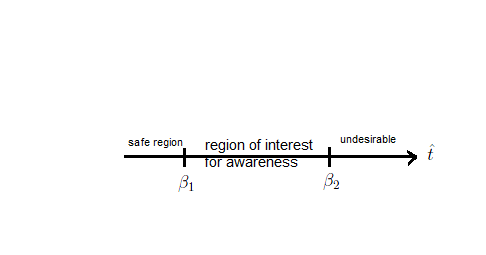
\includegraphics[scale=0.8]{awareness-line}};
\end{tikzpicture}&
\end{align*}
\begin{center}
\caption{Region segmentation for awareness}
\end{center}
\end{figure}

\begin{itemize}
\item 
For ${t_p}>>{t_c}$ vehicle is far away and both pedestrian and vehicle can just maintain their current speed. $\alpha_p$ = $\gamma,$ where $\gamma$ is considered to be fairly safe value for the system

\item 
For ${t_c}>>{t_p}$ this is undesirable and is a catastrophic scenario and not expected if the system is operational. $\alpha_p = 0$

\item
	Now considering some positive value $\beta_1$ and $\beta_2$ which gives a lower bound and upper bound of the ratio between $t_p$ and $t_c$. We are interested in evaluating the dynamics of \textit{awareness} within this value range ($t_p, t_c$). $\beta_1$ and $\beta_2$ can be mathematically shown as below. More on such a parameter can be found in \cite{yousef2016forward}.

	\begin{equation}
	\begin{array}{l@{}}
		\beta_1 \times {t_c} < {t_p} \\
		\beta_2 \times {t_c} > {t_p}
	\end{array}
	\end{equation}

	$\Omega(t_p, t_c)$ is defined as follows, where $\hat{t}$ is given by $\frac{t_p}{t_c}$\\
	\begin{empheq}[left=\empheqlbrace]{align}
		0, \hat{t} < \beta_1 \\
		\gamma, \hat{t} > \beta_2 \\
		\gamma \times \frac{\hat{t}}{\beta_2 - \beta_1}, \beta_1 > \hat{t} > \beta_1
	\end{empheq}

\end {itemize}

Considering the pedestrian and vehicle system always expected to be safe, LSTM cell state may be refined with calculated value for $\alpha_v$

%\pagebreak
\newpara
\textbf{Pedestrian bounding box location calculation:}
To aid the LSTM cell refinement because of vehicle movement and its change in direction we did some experiment. Below figures are some of the sample images captured during the experiment. %Assuming the vehicle from a constant distance from a virtual point on the x-axis in the image frame of reference.

\begin{figure}[H]
\begin{align*}
\begin{tikzpicture}[baseline=-1pt]
\node[] at (0,0) {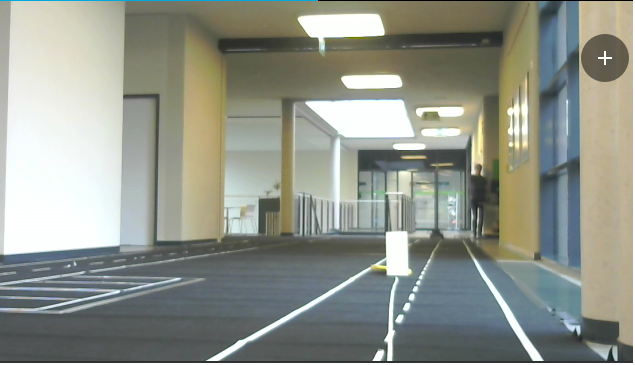
\includegraphics[scale=1.0]{6m339d}};
\end{tikzpicture}&
\end{align*}
\begin{center}
\caption{Vehicle's initial position }
\end{center}
\end{figure}

The above image was captured when an object (a whiteboard) was kept at a distance of 6m and 339-degree angle with the object.

\begin{figure}[H]
\begin{align*}
\begin{tikzpicture}[baseline=-1pt]
\node[] at (0,0) {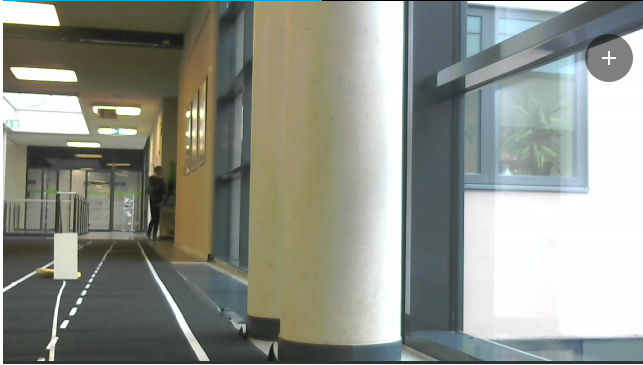
\includegraphics[scale=1.0]{6m14d_3_2cm}};
\end{tikzpicture}&
\end{align*}
\begin{center}
\caption{Vehicle's position after an angular movement}
\end{center}
\end{figure}

The above image was captured when an object was kept at a distance of 6m and 14-degree angle with the object.

Considering the below representation, a person represented as a bounding box in a frame by (x,y,w,h), where (x,y) is the center co-ordinate of the bottom edge of the bounding box and \textit{w} is the width of the bounding box and \textit{h} is the height of the bounding box. The position of the pedestrian bounding box in the next frame is  shown as ${P}_1$ in the below figure.

\begin{figure}[H]
\begin{align*}
\begin{tikzpicture}[baseline=-1pt]
\node[] at (0,0) {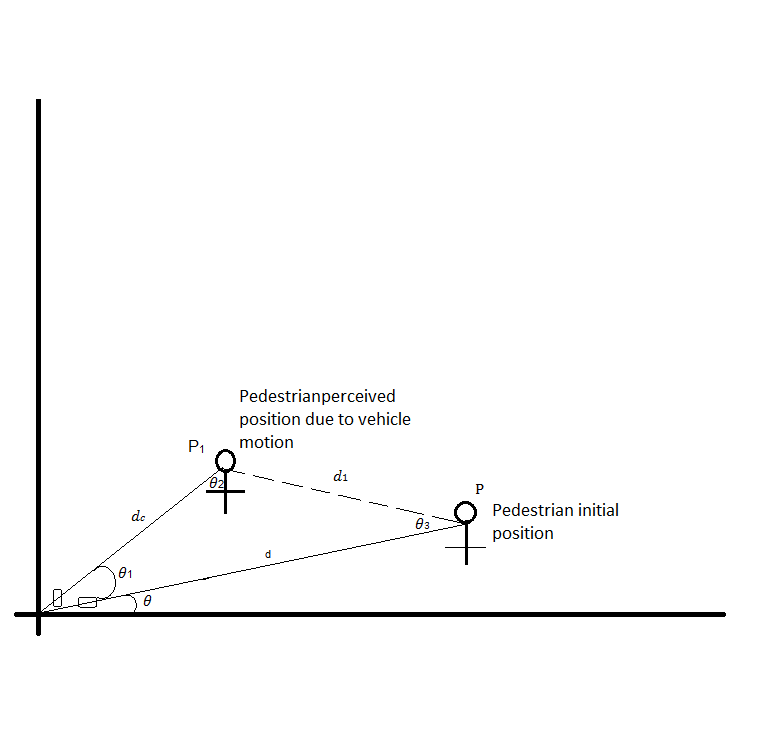
\includegraphics[scale=0.8]{Illustration-vehicle-motion}};
\end{tikzpicture}&
\end{align*}
\begin{center}
\caption{Illustration of the vehicle's angular motion}
\end{center}
\end{figure}

In the above figure, the expanded bounding box showed in the dashed-line to differentiate the change in dimension due to the vehicle motion.

\begin{equation}
\begin{array}{l@{}}
{P}=(x,y,w,h) \\
%{P}_{\hat{t}}=(x_{\hat{t}},y_{\hat{t}},w_{\hat{t}},h_{\hat{t}})
{P}_1=(x_1,y_1,w_1,h_1)
\end{array}
\end{equation}

%Where ${P}_{\hat{t}}$ is the position of the pedestrian at timestamp $(t+\Delta t)$, and $\Delta t$ is given by below equation.
Where ${P}_1$ is the position of the pedestrian at the next frame time stamp.
The next frame time stamp symbolically $\hat{t}$ is time-stamp at which the next frame is captured and can be given by below expression
\begin{equation} \label{delta-t}
\begin{array}{l@{}}
\hat{t} = t +  \Delta t \\
\Delta t = \frac{1}{fps}
\end{array}
\end{equation}


Where \textit{fps} is a measure of how many frames captured by the camera in one second

$(x_1,y_1,w_1,h_1)$ depends on basically three factors speed of the vehicle, speed of the pedestrian and the angle of rotation of the vehicle. Also, it is necessary to be noted that other social aspects such as obstacles, neighborhood pedestrian, a sudden change in pedestrian's own decision for the destination and displacement of the camera will have an impact.
Here we focused on the aspect of the vehicle's motion (speed and direction).


%A vehicle moving with a speed of $V_c$ shall travel a distance within \textit{a frame }time duration is given by the below equation.

%\begin{equation}
%d_v = \Delta t \times V_c
%\end{equation}

%A person moving with a speed of $V_p$ shall travel a distance within \textit{a frame }time duration is given by the below equation.

%\begin{equation}
%d_p = \Delta t \times V_p
%\end{equation}

%The new coordinates $(\hat{x}, \hat{y})$ for the pedestrian in the image frame of reference is given by

%\begin{equation}
%\begin{array}{l@{}}
%x_{\hat{t}} =x_t + \frac{d_p cos\theta }{CF}\\
%y_{\hat{t}} =y_t + \frac{d_p sin\theta }{CF}
%\end{array}			
%\end{equation}

%Where $\theta$ is the angle of the pedestrian movement \\
%CF is the calibration factor of the camera and used for scale conversion.

%Assuming the initial position of the pedestrain (x,y) on the ground frame-of-reference and due to this change of distance $\Delta d_v$ and $\Delta d_p$, the resultant distance and angle between vehicle and pedestrian shall be changed and given by below relation. Considering the car camera coordinate in the previous frame at the origin, it moves always in the direction of \textit{y-axis}, its new co-ordinate at $\hat{t}$ shall be $(x_0, d_v)$. New position of the pedestrian shall be $(x + d_p cos\theta, y + d_p sin\theta)$

%Assuming the initial position of the pedestrian (x,y) on the ground frame-of-reference and due to this change of distance $\Delta d_v$ and $\Delta d_p$, the resultant distance between vehicle and pedestrian shall be changed and given by below relation. Considering the car camera coordinate in the previous frame at the origin, it moves always in the direction of \textit{y-axis}, its new co-ordinate at $\hat{t}$ shall be $(x_0, d_v)$. New position of the pedestrian shall be $(x + d_p cos\theta, y + d_p sin\theta)$


%\begin{equation}
%\begin{array}{l@{}}
%d_{\hat{t }} =\sqrt{(x_0 - x-d_p cos\theta)^2 + (d_v - y-d_p sin\theta)^2} \\
%\hat{\theta}= tan^-1\frac{(y-d_v)}{(x-x_0)} \\
%\end{array}
%\end{equation}


%Consider the mid point ($P$) of the lower side of the pedestrian bounding box as the initial position of the pedestrian (x,y) on the image frame-of-reference.
\textbf{Effect of vehicle angular motion:} \\
Consider ($P$) as the center of the lower edge of the pedestrian bounding box as the initial position of the pedestrian with co-ordinate (x,y) on the image frame-of-reference and (w,h) as bounding box width and height respectively.

%, the initial angle between camera and pedestrain can be approximated as

%\begin{equation}
%{\theta }= tan^-1\frac{(y-y_0)}{(x-x_0)}
%\end{equation}

%\textit{Note:} Some image processing software package considers top-left corner as (0,0) and some others consider bottom-left corner as (0,0). For the simplicity purpose we assumed  bottom-left corner as (0,0).

%\pagebreak
For the YAW-motion of the camera, we have observed from the experiment that, with the camera angular motion, the particular object makes a horizontal displacement. And the magnitude of this displacement is approximated with the amount of the camera rotation. This displacement depends on the following factors, the angle of view of the camera measured in degrees, and the frame width measured in pixel. Mathematically, the displacement of the bounding box can be given as below

\begin{equation} \label{yaw-displacement}
{d_{yaw}} = \pi({\theta , fw, \alpha})
\end{equation}

Where ${d_{yaw}}$ is the displacement in the image measured in pixel due to camera rotation ${\theta}$ degrees, and $fw$ is the frame width measured with a number of pixels, and $\alpha$ is the angle of view.

It is also noted that for the counter-clockwise motion the object makes a left-to-right displacement and the reverse for a clockwise motion. 

Considering the cameras angle of view $\alpha$ (in degrees), which is given by the below equation
\begin{equation} \label{angle-of-view}
\alpha =2\arctan {\frac {d_s}{2f}}
\end{equation}
where ${d_s}$ is the sensor dimension and $f$ is the focal length. Both are measured in $mm$.
% https://en.wikipedia.org/wiki/Angle_of_view

The visible part of the scene (within the angle of view) is represented by the frame with $fw$. Now, the displacement due to angular movement can be expressed as
\begin{equation} \label{yaw-displacement-detail}
{d_{yaw}} = \frac {fw}{\alpha} \times {\theta}
\end{equation}

Considering a camera with AoV 90$^{\circ}$ and image width of the produced image as 720 pixels, we find for angular rotation of 15$^{\circ}$, the displacement is 120 pixels. \\
 
The modified position of P due to displacement ${d_{yaw}}$ is expressed as
\begin{equation} \label{new-xy}
(x_1, y_1) = (x + d_{yaw}, y)
\end{equation}
$(x_1, y_1)$ is the anticipated position in the image frame of reference, in the unit of pixel.
A point to be noted, there is a minute change in the inclination of the top and bottom edges of the bounding box due to the YAW-motion of the camera as seen in the experiment, and in the above equation it is neglected for the estimation.

%Using the given equation in \cite{dougan2010real}, which tries to estimate the instantaneous velocity vector of a point (in 2D space) using displacement vector which depends upon the scale of the image, frame rate, and vehicle speed.
%\begin{equation} \label{conversion}
%{v}= \frac{\delta p}{\delta t}
%\end{equation} 
%v is the instantaneous velocity vector \\
%${\delta p}$ displacement vector, displacement vector measured in pixel units \\
%${\delta t}$ is the frame capture rate

%The magnitude of this vector in image space is transformed into object space using a scale factor as described below. Scale factor (${\lambda}$) related to distance between camera and object and the focal length of the camera.

%Object space displacement can be computed as below

%\begin{equation} \label{conversion}
%{d_o}= {d_i} \times \lambda
%\end{equation} 

%where $d_o$ represents the distance in object space \\
%$d_i$ represents the displacement in image space \\
%${\lambda}$ is the scale factor of the camera that converts real-world distance to distance in image space, it is is a function of camera's focal length and camera-object distance discussed in \cite{dougan2010real}, expressed as below relation.

%\begin{equation} \label{sf-precompute}
%\lambda \cong 1 + \frac{d}{f}
%\end{equation}

%d is the distance between camera and object and f is the focal length of the camera. Consider a fixed focal length for the camera in a particular setting $\lambda$ is a function of camera-object distance and shall be precomputed. % to be applied in the equation \ref{object-distance}

%When the vehicle moves with an angle ${\theta }$ in a time period ${\Delta t}$, the point P now displaced by the same angle as ${\theta}$.

\textbf{Effect of vehicle linear motion:} \\
Consider the $d$ is the current distance between the vehicle and the pedestrian, which can be found by using the midpoint of the bottom edge of the detected bounding box \cite{CarND-Advanced-Lane}. After performing a perspective transformation, its position on the warped image can be calculated. From the warped image, the pixel position can be correlated with the distance in meter(SI unit). The change in the distance after a frame time due to vehicle movement is computed as below. Consider the vehicle speed \textit{v}, a vehicle moves a distance $d_v$ in a frame time period $\Delta t$ is given by the below equation and measured in the SI unit.
\begin{equation} \label{distance-in-pixel}
{d_v}= v \times \Delta t
\end{equation} 


% the displacement of the point \textit{P} on the image is given by

 %object space displacement can be converted to image space by dividing it with the scale factor. 
%\begin{equation} \label{distance-in-pixel}
%{d_1}= \frac{v \times \Delta t}{\lambda}
%\end{equation} 

%\pagebreak
%Where ${\lambda}$ is the scale factor, ${d_1}$ is the displacement in image space, $\Delta t$ as given in \ref{delta-t}. This equation gives the metric displacement (${d_1}$) amount in the image space and can be converted to the number of pixels units using dimensions of effective image area and pixel size.

%Now to determine this translated point ${P_1}$ in the below figure, laws of sine is used as given below.

%\begin{equation}
%\frac{d_1}{sin \theta_1} = \frac{d}{sin \theta_2} 
%\end{equation}

%In the above equation, $\theta_1$ is the angle made by vehicle, $\theta_2$ is the only unknown, after finding that $\theta_3$ can be easily found.

%By applying same laws of sine, the distance $d_c$ (from the imaginary vehicle point to the point $P_1$) in pixels can be evaluated from the below equation.

%\begin{equation} \label{camera-distance}
%\frac{d_c}{sin \theta_3} = \frac{d}{sin \theta_2} 
%\end{equation} 

%The resultant angle between vehicle and pedestrian, ${\hat{\theta}}$ can be expressed as below.
%\begin{equation} \label{theta-large}
%\begin{array}{l@{}}
%\hat{\theta } = \theta  + {\theta}_1
%\end{array}			
%\end{equation} 

%Where ${\theta}$ is the initial angle between vehicle and pedestrian and ${{\theta}_1}$ is the angle made by the vehicle.

%The coordinates of point ${P_1(x_1, y_1)}$ can be formulated as
%\begin{equation} \label{new-xy}
%\begin{array}{l@{}} 
%x_1 = d_c cos \hat{\theta } \\
%y_1 = d_c sin \hat{\theta } 
%\end{array}			
%\end{equation} 
%\label{new-xy}

%Where $d_c$ is given as in equation \ref{camera-distance} and $\hat{\theta}$ in \ref{theta-large}

%The distance between camera and object at ${\hat{t}}$𝑡is given as below
%\begin{equation} \label{object-distance}
%d_{\hat{t}} = d_c \times {\lambda} + K
%\end{equation}

%where $d_c$ is the measured distance in image space as in \ref{distance-in-pixel}, can be measured using any %distance metric like inch or SI unit \\
%${\lambda}$ is the scale factor, K is the constant distance that is not captured within the vehicle's camera and usually known as \textit{blind spot}. 
%$\hat{d_c}$  is the least distance between the camera and the point in the ground that is captured in the image% frame, in the object space and measured in SI unit(e.g m). 

%The distance to an object \cite{jungel2007improving} can be determined from size of the object in the image space and the focal length of the camera. The distance between camera and object in the scene can be derived by below equation.

%\begin{equation} \label{distance-camera-object}
%d_{object} = \frac{w \times f}{p}
%\end{equation} 

%where $d_{object}$ is the distance between camera and object, \textit{w} corresponds to width of the object, \textit{f} represents the focal length of the camera and \textit{p} is the perceived width in the image space.

%\pagebreak
%Due to the angular rotation ${\theta}_1$, the bottom right point of the bounding box (x+w, y-h) is translated using the linear transformation as below \\
 
%\begin{equation} \label{rotaion-translation}
%(w_1, h_1) = (x+w, y-h) 

%\[ 
%\begin{bmatrix}
%w_1 & h_1
%\end{bmatrix}
%=\begin{bmatrix}
%cos \theta_1 & -sin \theta_1\\
%sin \theta_1 & cos \theta_1
%\end{bmatrix}
%\begin{bmatrix}
%x+w &  y-h
%\end{bmatrix}
%\]

%\end{equation

%So with a moving camera, modified perceived width and height in pixel represented as ${p_w}$ ${p_h}$ respectively given by below expression where $w_s$ and $h_s$ are the standard width and height of a pedestrian and used as a constant.

%\begin{equation} \label{new-height-width-pixels}
%\begin{array}{l@{}}
%{p_w} = \frac{w_s \times f}{d_{\hat{t}}} \\
%{p_h} = \frac{h_s \times f}{d_{\hat{t}}}
%\end{array}			
%\end{equation} 

The distance between the camera and object in the scene can be derived by the below equation.
\begin{equation} \label{distance-camera-object}
d_o = \frac{w_o \times f}{w}
\end{equation}
where $d_o$ is the distance between camera and object, $w_o$ corresponds to the width of the object in the object space, f represents the focal length of the camera and $w$ is the perceived width of the object. \\
$d_o$, $w_o$, $f$, $w$ are measured in SI units and $w$ can be converted to a number of pixels using the image specification.

So due to the vehicle's linear movement, ${w_1}$, ${h_1}$ are the modified perceived width and height in the image respectively, calculated using \ref{distance-camera-object} and given as below

\begin{equation}
\begin{array}{l@{}} 
{w_1} = \frac{d}{d-d_v} \times w \\
{h_1} = \frac{d}{d-d_v} \times h
\end{array}
\end{equation}
Where $d$ is the distance between camera and object computed from the pedestrian bounding box and $d_v$ is the distance covered by the vehicle in a frame time. $(w,h)$ are the width and height of the bounding box as measured from the image in number of pixels. $(w_1,h_1)$ are the modified perceived width and height of the bounding box in the number of pixels.

Combining the above results with equation \ref{new-xy}, the midpoint of the bottom edge of the pedestrian bounding box is approximated as $({x_1}, {y_1})$ and the modified dimension for width and height as $({w_1}, {h_1})$, which helps in LSTM state refinement.

%\comment{
%}

\section{Object detection: SSD}
After image data acquisition and data preparation, the challenging task remains, how to train the model. To better understand the SSD framework and training steps, a flowchart is prepared that detailed it's workings.
 % In the current work and by other authors also the term \textit{training }and \textit{learning}are used interchangeably. 
\begin{figure}[H]
\begin{center}
\begin{tikzpicture}[
    node distance = 5mm and 20mm,
      start chain = going below,
     arrow/.style = {thick,-stealth},
      base/.style = {% common features of all nodes
            draw, thick, 
            minimum width=30mm, minimum height=10mm, align=center,
            inner sep=1mm, outer sep=0mm,
            on chain, join=by arrow},
  decision/.style = {diamond, base,
            aspect=1.7, inner xsep=0mm},
   process/.style = {rectangle, base},
 startstop/.style = {rectangle, rounded corners, base},
 stop/.style = {rectangle, rounded corners},
                        ]
\node (start) [startstop] {Start};
\node (0) [process]{Image data preparation}; 
\node (1) [process]{Default bounding boxes}; 
\node (2) [process]{ Offsets is predicted}; 
\node (3) [process]{ Per-class score prediction}; 
\node (4) [process]{Ground truth box and default box matching };
\node (5) [process]{ Default-box and ground truth matching}; 
\node (6) [process]{ Combined loss function and back propagation}; 
\node (sevralepocs) [process]{ Train for several epochs}; 
\node (7) [process]{ Validate and save the model};
\node [decision] (validation) { val-error accepted?};
\node (end)  [startstop, below=5mm of validation]  {END};

\draw [arrow] (validation.west) to node [] {No} + (-3,0) |-  (sevralepocs.west);
\path (validation) to node []{Yes} (end);

\end{tikzpicture}
\begin{center}
\caption{Flowchart for SSD network training}
\end{center}
\end{center}
\end{figure}

Image data is prepared with data augmentation. A set of default bounding boxes associated with each feature map cell is calculated. At each feature map cell, offsets relative to default box shapes in the cell is predicted.
Each ground truth box is matched with the default box with best jaccard overlap. The default box is matched to any ground truth with jaccard overlap greater than 0.5. After the model is trained, its accuracy and performance are measured and that is described in detail in the subsequent chapters.

\subsection{Network architectures}
Below depicted the details of the convolution in image and CNN building blocks.

\begin{figure}[H]
\begin{align*}
\begin{tikzpicture}[baseline=-3pt]
\node[] at (0,0) {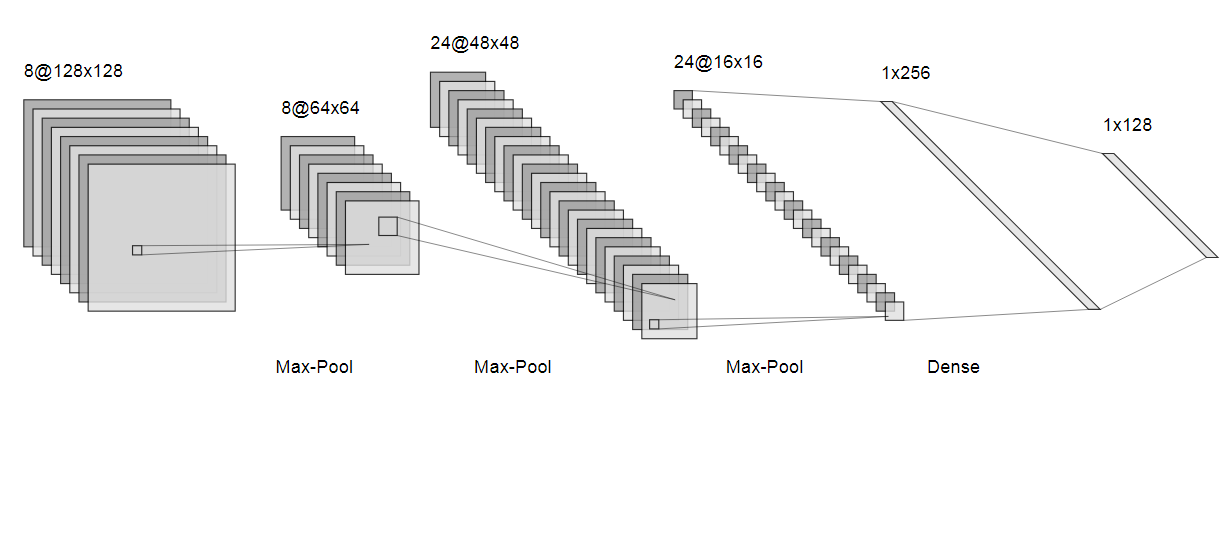
\includegraphics[scale=0.5]{LeNet-Arch}};
\end{tikzpicture}&
\end{align*}
\begin{center}
\caption[Architecture of a traditional convolutional neural network.]{The architecture of the original convolutional neural network, as introduced by LeCun et al. (1989), alternates between convolutional layers including hyperbolic tangent non-linearities and subsampling layers. In this illustration, the convolutional layers already include non-linearities and, thus, a convolutional layer actually represents two layers. The feature maps of the final subsampling layer are then fed into the actual classifier consisting of an arbitrary number of fully connected layers. The output layer usually uses softmax activation functions. \footnote{http://alexlenail.me/NN-SVG/LeNet.html}}
	\label{fig:traditional-convolutional-network}
\end{center}
\end{figure}

\begin{itemize}
\item
\textbf{First Layer:} A convolution layer with depth 8, height 128, width 128 and filter size(8,8)
\item
\textbf{Second Layer:} Max-Pool layer
\item
\textbf{Third Layer:} A convolution layer with depth 8, height 64, width 64 and filter size(16,16)
\item
\textbf{Fourth Layer:} Max-Pool layer
\item
\textbf{Fifth Layer:} A convolution layer with depth 24, height 16, width 16 and filter size(8,8)
\item
\textbf{Fifth Layer:} A convolution layer with depth 24, height 16, width 16 and filter size(8,8)
\item
\textbf{Sixth and seventh Layer:} Are dense layers
\end{itemize}

\newpara \textbf{Convolution layer} It is the first layer to which the input image is given. A small matrix otherwise known as a filter or kernel moves along the image and is convoluted with the input image. As a process of convolution, kernel elements are multiplied with the original pixel value and these values are summed up and produce a feature map as input for further layers.
 
\newpara \textbf{Nonlinear layer}
A non-linearity is added to the output generated from a convolution layer in the form of an activation function in this layer. The basic idea of adding a non-linear layer is to make different layers within the network to have a non-linear relationship and this ensures the network can make more complex decisions.
Usually, ReLU is used as a non-linear activation function and mathematically given as below.
%https://machinelearningmastery.com/rectified-linear-activation-function-for-deep-learning-neural-networks/

\begin{equation}
	f(x) =max(0, x)
\end {equation}
Where x is the input to a neuron and output is similar to a ramp function.
Although simple, it has been demonstrated that this activation function enables better performance in deeper networks compared to widely used complex functions such as \textit{sigmoid} (fig:\ref{fig:Sigmoid-function}) and \textit{hyperbolic tangent}. % (fig: \ref{fig:tanh-function}).

\newpara \textbf{Pooling layer}
The subsequent layer after the non-linear layer. It downsamples the image, as a result, the processed image volume is reduced. Max-pooling is similar to convolution, but it chooses the maximum element within the area where the max pool filter is applied. For a pooling size (2,2) the input is halved in both spatial dimensions.

\newpara \textbf{Fully connected layer}
Normally a fully connected layer is attached to the Network as the last layer of the Network. The fully connected layer performs classification by taking input as features extracted and transformed in the previous \textit{conv-relu-pooling} layers. This results in an N-dimensional vector, where N is the number of classes the model is trained on.

\newpara CNN learns the filters that traditional image classification algorithm handcrafts. This makes CNN less pre-processing compared to other traditional algorithm and results in superior results. There are many evolution of CNNs starting from LeNet (LeCun et al., 1989) for zip code recognition, LeNet-5 (1998) a 7 layer CNN \ref{fig:traditional-convolutional-network} by LeCun et al. for handwritten numbers on the check recognition, AlexNet by Alex Krizhevsky et al. in 2012 used deeper layers and more filters per layer than leNet-5. It also used ReLU activation, max pooling, dropout, data augmentation and SGD with momentum during training. \footnote{These terms shall be discussed in the subsequent chapter.} This achieved a record-breaking result at that time. ZFNet in 2013 was the winner of ILSVRC 2013 with a small tweaking to AlexNet. 2014, GoogleNet is otherwise known as Inception V1 from Google achieved human-level performance. Another net in the same year got the attention known as VGGNet. It uses only 3x3 convolution, 16 layers and lots of filters. It consists of 138 million parameters which were one of the major disadvantages and required more time to train. The weight configuration of this is publicly available and used as a baseline feature extractor.

%Standard CNN architectures, over the last 2 decades uses set of standard layer that can be graphically \ref{tomepel} represented as below. 

%\begin{figure}[H]
%\begin{align*}
%\begin{tikzpicture}[baseline=-3pt]
%\node[] at (0,0) {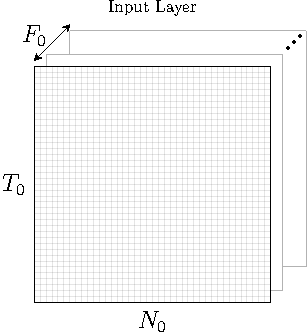
\includegraphics[scale=0.5]{input_layer}};
%\end{tikzpicture}&=
%
%\begin{tikzpicture}[baseline=-0pt]
%\draw (0,-1) rectangle (0+0.3,1);
%\node[align=center,scale = 0.65] at (0+0.15,0) {I \\ n \\ p \\ u \\ t};
%\end{tikzpicture}\;,&
%
%\begin{tikzpicture}[baseline=-3pt]
%\node[] at (0,0) {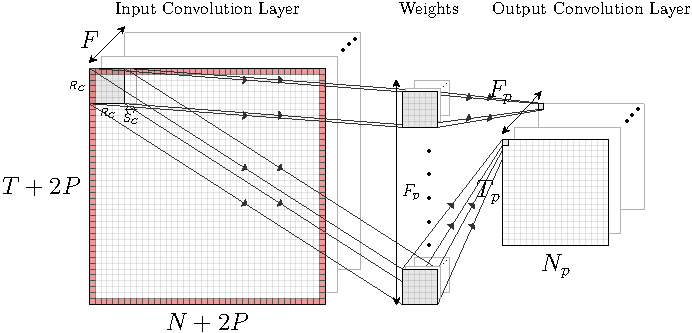
\includegraphics[scale=0.5]{VGG-conv}};
%\end{tikzpicture}&=
%
%\begin{tikzpicture}[baseline=-0pt]
%\filldraw[fill=blue!30!white] (0,-1) rectangle (0+0.3,1);
%\node[align=center,scale = 0.65] at (0+0.15,0) {C \\ o \\ n \\ v};
%\end{tikzpicture}\;,\notag\\
%
%\begin{tikzpicture}[baseline=-3pt]
%\node[] at (0,0) {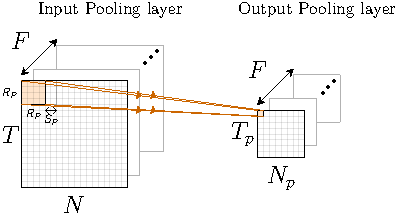
\includegraphics[scale=0.5]{VGG-pool}};
%\end{tikzpicture}&=
%
%\begin{tikzpicture}[baseline=-0pt]
%\filldraw[fill=red!30!white] (0,-1) rectangle (0+0.3,1);
%\node[align=center,scale = 0.65] at (0+0.15,0) {P \\ o \\ o \\ l};
%\end{tikzpicture}\;,&
%
%\begin{tikzpicture}[baseline=-3pt]
%\node[] at (0,0) {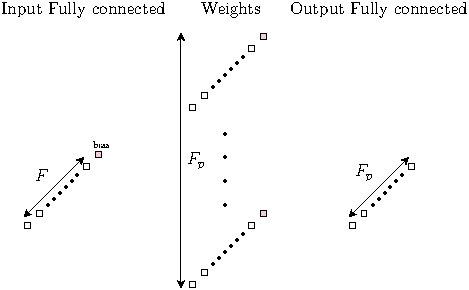
\includegraphics[scale=0.5]{VGG-fc}};
%\end{tikzpicture}&=
%
%\begin{tikzpicture}[baseline=-0pt]
%\filldraw[fill=green!30!white] (0,-1) rectangle (0+0.3,1);
%\node[align=center,scale = 0.65] at (0+0.15,0) {F \\ u \\ l \\ l};
%\end{tikzpicture}
%\end{align*}
%\begin{center}
%\caption{CNN layers: Schematic representation, source:Thomas Epelbaum GitHub}
%\label{fig:Schematic-representation}
%\end{center}
%\end{figure}

%\newpara Based on these schematic layers, a simple graphical \footnote{\label{tomepel} Images source: Thomas Epelbaum GitHub: https:\textbackslash github.com\textbackslash tomepel\textbackslash Technical\_Book\_DLaccessed on 07th August 2019 } representation of VGG-Net is shown below.
%\begin{figure}[H]
%\begin{center}
%\begin{tikzpicture}
%\node[] at (0,0) {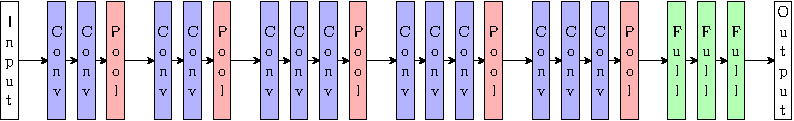
\includegraphics[scale=1]{VGG}};
%\end{tikzpicture}
%\caption{VGG-Net, souece: Thomas Epelbaum GitHub}
%\end{center}
%\end{figure} 

\section{Terminology}
Some of the key concepts that are studied and useful are presented in subsequent texts.

\subsection{Data Augmentation}
Data augmentation is a key in image-based deep learning application. This makes the model robust to different object sizes, logically achievable  additional training image generation via application of various image modifications such as flipping horizontally \footnote{Many time flipping the image vertically does not make sense in real-world scenarios, wherever it makes sense, it can be done as well.}, shear, distortion, change in color intensity. In \cite{liu2016ssd} authors mentioned the application of flipping each image randomly horizontally with the probability of 0.5, this ensures objects appear on left and right with similar likelihood.

\subsection{Non-Maximum Suppression (NMS)}
During inference time, SSD predicts, a large number of boxes in a cluttered manner. To prune most of them, a technique called \textit{non-maximum suppression} is applied. This technique discards those boxes having label confidence less than a threshold and IoU less than a defined threshold. \footnote{Usually 0.45 is used as IoU threshold}. After discarding such boxes, only top \textit{N} predictions are returned which ensures most likely predictions.
\subsection{Epoch:}
During the learning, the network sees the set of samples several times. During the training, presenting the network entire set of samples once is known as an epoch. So an epoch represents one iteration over the entire dataset.
\subsection{Batch and batch size:}
Mainly because of two reasons we can not pass the entire dataset to the network for the training purpose at once. Firstly, datasets by nature most of the time are huge. Let it be image data or some other textual data, in many scenarios it is not possible to feed all the data because of hardware constraints, such as not enough RAM to hold the entire dataset.
Secondly, to update weight during the training process, the network has to wait for a very very long time to calculate the delta weight after processing all the input data. To solve this problem usually the full dataset is split into several small batches and the number of samples within each small batch is known as 
Batch and batch size.

\subsection{Iterations:} 
Number of batches that a neural network process to complete a single epoch.
The number of  iterations, batch size and  number of data samples in the dataset is given by, the below expression.
\begin{equation}
    D = B * I
\end{equation}
Where D is the total number of samples in the dataset.
\\*B is the number of samples in the mini-batch that is fed to the network at once.
\\*I is the  total number of batches the network process in a single epoch.

Larger batch size requires more computational resources and achieves faster completion, in contrast, smaller batch size leads to more generalization. In this regards, Yann  LeCun humorously said
\begin{quote}
``Training with large mini-batches is bad for your health. More importantly, it's bad for your test error.  Friends, don't let friends use mini-batches larger than 32.''
\end{quote}   

The empirical study of the performance of mini-batch stochastic gradient descent in \cite{masters2018revisiting} show that, the team obtained the best training stability and generalization performance using small batch sizes, for a given computational cost, across a wide range of experiments they conducted. In all cases, they have achieved the best results with batch sizes m = 32 or smaller.

\subsection{Intersection Over Union:}
Intersection Over Union (IOU) is a measure similar to the Jaccard Index that measures the overlap ratio between two bounding boxes. It evaluates the ratio between the area of overlap between two BBs and the area of union between them.

\begin{equation}
    IoU = \frac{area\: of\: overlap} {area\: of\: union} =
\end{equation}

\begin{center}
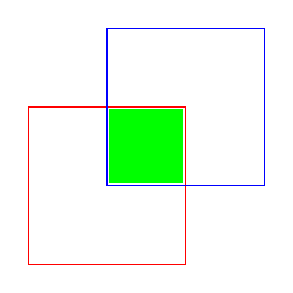
\begin{tikzpicture}
\draw [red] (0, 0) rectangle (2, 2);
\draw [blue] (1.0, 1.0) rectangle (3.0, 3.0);
\begin{scope}
	\fill[green] (1.03, 1.03) rectangle (1.97, 1.97);
\end{scope}
\end{tikzpicture}

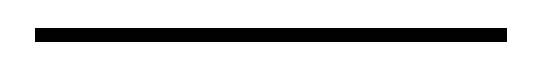
\begin{tikzpicture}
    \draw[line width=5pt,fill=black] (0,2) -- (6,2);
\end{tikzpicture}\vspace{0.2cm}%

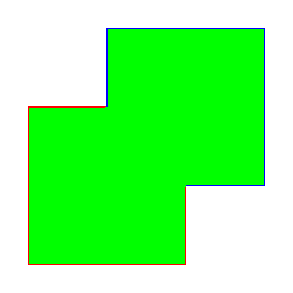
\begin{tikzpicture}
    \filldraw [draw=red,fill=green] (0, 0) rectangle (2, 2);
    \filldraw [draw=blue,fill=green] (1.0, 1.0) rectangle (3.0, 3.0);
    %\begin{scope}
			\fill[green] (0.98, 0.98) rectangle (2.0, 2.0);
		%\end{scope}
\end{tikzpicture}
\end{center}

